\chapter{Experiments and Results}
\label{ch:Experiments}

In this chapter we introduce all performed experiments. This includes a general experimetal setup, as well as more detailed experiment settings including their results.

Since our work is twofold, we start with the experiments regarding the replication of the PGExplainer with a changed downstream model architecture and a focus on the inductive setting in Section \ref{sec:experiments_replication}. Next, we describe the experiments performed on the adapted explainer framework to generate explanations for the NeuroSAT model predictions of unsatisfiable problems in Section \ref{sec:SAT-experiments}.

\section{Replication of PGExplainer}
\label{sec:experiments_replication}
In this section we present all experiments regarding the replication of the presented explainer model. We first present the common experimental setup, including the datasets, corresponding downstream models and hyperparameter searches. In Section xy we replicate the experiments in the inductive setting from the original paper. We also include a study of the effect of using a larger set of training data, as the original proposes that only few training instances are necessary for the explainer to generalize well. Furthermore, we perform the original quantitative experiment in the collective setting with the found hyperparameters for better comparability, as this was the core study of the original paper. In Section xy we run an experiment specific to the BA-2Motif dataset, as we found that it behaves opposite to the expectations. Later, we study the effects of the specific node sets that were used in the original codebase in Section xy. Lastly, we qualitatively evaluate the explanations provided by our reimplemented model (see Section xy).

\subsection{Common experimental setup}
\label{sec:PGE_exp_setup}
In this section we describe the common setup for the experiments that we perform on PGExplainer.
We follow the experimental setup from the PGExplainer as closely as possible. Since the textual description refers to the setup from GNNExplainer and is lacking in some aspects, we extract the missing information from the codebase. As the hyperparameters are unclear or not comprehensible for some tasks we also draw information from the configs of the replication by Holdijk et al. \cite{holdijk2021re}.

\textbf{Datasets}\par
We perform the experiments on the same datasets used in the original. These were constructed by the authors similarly to the ones used in the baseline GNNExplainer. Four synthetic datasets were used for the node classification tasks. For the graph classification task the authors provide one synthetic dataset as well as the real-world dataset MUTAG. The synthetic datasets are constructed by creating a base graph and attaching motifs to random nodes of the base graph. These motifs determine the labels of the nodes or graphs, depending on the task at hand, and therefore serve as the ground truth explanations that the explainer shall detect. Statistics of each dataset can be found in Table \ref{tab:dataset-statistics} and a visualization in Section \ref{sec:data_vis}. We will give a short description of each dataset. \bigskip

Since three of the synthetic datasets use a Barabási-Albert (BA) graph as a base, we briefly introduce the BA model. The BA model generates scale-free networks that grow over time. Starting with an initialization network of $m_0 \geq m$ nodes, at each step a new node is added and connected to $m$ of the nodes already existing in the graph. The probability for each node to be selected as a neighbor depends on its degree, leading to a higher probability for nodes that already have a high degree rather than nodes with a low degree \cite{albert2002statistical}. \bigskip

BA-Shapes is the first node dataset that consists of a single BA-graph with 300 nodes and 80 "house" motifs - five nodes resembling the shape of a house (TODO: see xy). Base graph nodes are labeled with 0 while nodes at the top/middle/bottom of the "house" are labeled with 1,2,3, respectively. The top node of each house motif is attached to a random base graph node. Additional edges are added for perturbation. Each node is assigned a 10-dimensional feature vector of 1s.

BA-Community consists of two unified BA-Shapes graphs. The features of the nodes are sampled from two Gaussian distributions. Nodes are labeled as in BA-Shapes for each community respectively, leading to 8 classes in total.

Tree-Cycles uses an 8-level balanced binary tree as a base graph. 80 cycle motifs, consisting of a 6 node cycle, are attached to random nodes from the base graph. Node features are assigned as a 10-dimensional vector of 1s. A node of the base graph is labeled as 0 and a motif node is labeled as 1.

The Tree-Grid dataset is assembled in the same way as Tree-Cycles, with the difference that the motifs are 3-by-3 grids. Node features and labels also follow the same procedure.
BA-2Motif is the first graph dataset with 800 graphs. Each of these graphs is obtained by attaching either a "house" or a cycle as a motif to a base BA graph with 20 nodes. According to the attached motif the graphs are assigned one of two labels, with 0 or 1 implying a house or circle, respectively.

The real-world dataset MUTAG contains $4,337$ molecule graphs that are assigned to one of 2 classes, depending on the molecules mutagenic effect \ref{}. Node features are assigned as a one-hot encoding in $\{0,1\}^{14}$, representing the chemical group of a node out of 14 possible ones. Following \ref{}, carbon rings with chemical groups $NH_2$ or $NO_2$ are known to be mutagenic, with carbon rings in general existing in both mutagenic and non-mutagenic graphs. The authors thus propose treating the carbon ring as a shared base graph and $NH_2$ and $NO_2$ as motifs for mutagenic graphs. Since there are no explicit motifs for the non-mutagenic graphs, these grapgs are not considered in PGExplainer.

\begin{table}[h]
    \centering
    \scriptsize
    \begin{tabular}{l|cccc|cc}
    \hline
    \textbf{} & \textbf{BA-Shapes} & \textbf{BA-Community} & \textbf{Tree-Cycles} & \textbf{Tree-Grid} & \textbf{BA-2motifs} & \textbf{MUTAG} \\
    \hline
    \#graphs & 1 & 1 & 1 & 1 & 1,000 & 4,337 \\
    \#nodes  & 700 & 1,400 & 871 & 1,231 & 25,000 & 131,488 \\
    \#edges  & 4,110 & 8,920 & 1,950 & 3,410 & 51,392 & 266,894 \\
    \#labels & 4 & 8 & 2 & 2 & 2 & 2 \\
    \hline
    \end{tabular}
    \caption[Statistics of PGExplainer datasets]{Dataset statistics for Node and Graph Classification tasks, reprinted from \cite{luo2020parameterized}.}
    \label{tab:dataset-statistics}
\end{table}

Note that in the collective setting used in the original paper the explainer is trained and evaluated on the same data. This data is further reduced by only using graphs and nodes that contain a ground truth motif. This makes sense for evaluation, since the AUROC cannot be calculated for ground truths with only one class present. However, the authors do not specify why the training is performed only on these instances. Therefore, only the 1,015 mutagenic graphs where either $NH_2$ or $NO_2$ are present are selected for the MUTAG experiment. \bigskip

\begin{figure}[h]
    \centering
    % First 3 images
    \begin{subfigure}[b]{0.2\textwidth}
        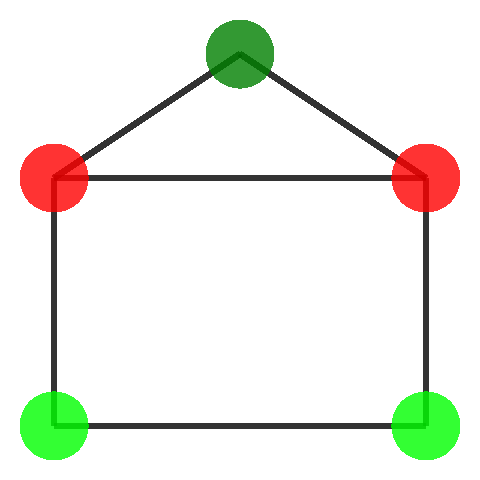
\includegraphics[width=\linewidth]{img/Motif_Vis/BA-Shapes-MOTIF.pdf}
        \caption{House motif}
    \end{subfigure}
    \begin{subfigure}[b]{0.2\textwidth}
        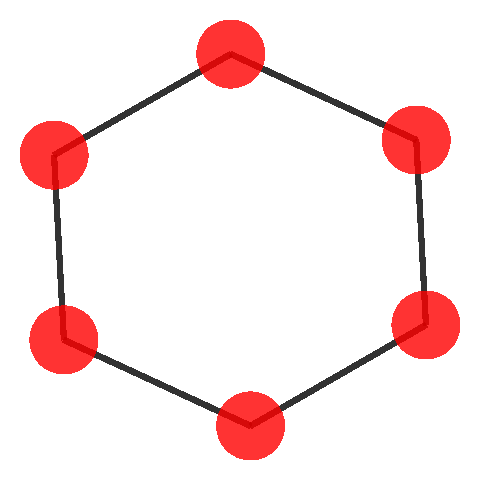
\includegraphics[width=\linewidth]{img/Motif_Vis/Tree-Cycles-MOTIF.pdf}
        \caption{Circle motif}
    \end{subfigure}
    \begin{subfigure}[b]{0.2\textwidth}
        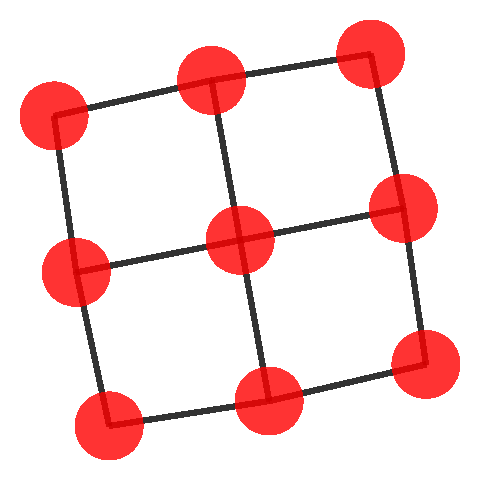
\includegraphics[width=\linewidth]{img/Motif_Vis/Tree-Grid-MOTIF.pdf}
        \caption{Grid motif}
    \end{subfigure}
    % Fourth image composed of two smaller images
    \begin{subfigure}[b]{0.30\textwidth}
        \centering
        \begin{subfigure}[b]{0.48\linewidth}
            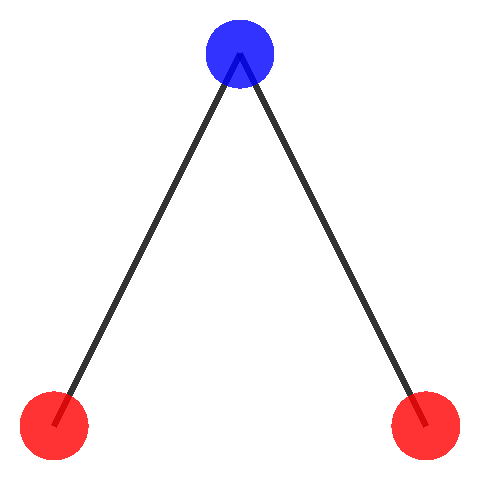
\includegraphics[width=\linewidth]{img/Motif_Vis/MUTAG-MOTIF1.pdf}
        \end{subfigure}
        \begin{subfigure}[b]{0.48\linewidth}
            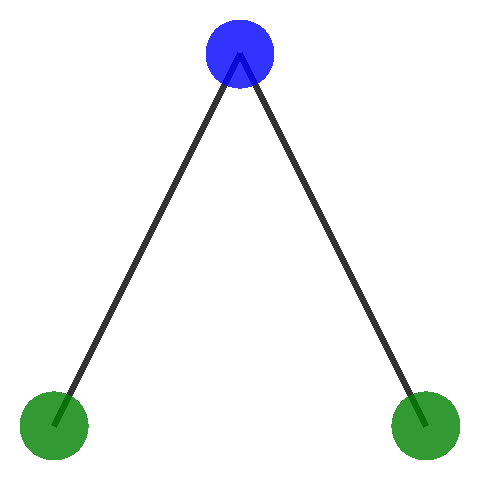
\includegraphics[width=\linewidth]{img/Motif_Vis/MUTAG-MOTIF2.pdf}
        \end{subfigure}
        \caption{$NO_2$ and $NH_2$ motifs}
    \end{subfigure}
    
    \caption{The different motifs used in the datasets.}
    \label{fig:motifs}
\end{figure}

In the node classification experiments the node sets containing instances used for training and evaluation were further finetuned per dataset. This leads to a selection of either all nodes that are part of a motif, or only one node per motif. This inconsistency is also left unexplained by the authors and extracted from the codebase. We perform an experiment on the effects of these node selections in \ref{sec:motif_set_experiment}.

For the motif node set used in BA-community multiple configurations exist in the PGExplainer codebase. One is extracted from the GNNExplainer \cite{ying2019gnnexplainer} and consists of the same nodes used for the BA-Shapes dataset, which seems unjustified and is not addressed in the paper. Another setting uses all motif nodes of both communities - effectively all nodes that do not belong to the two community base graphs:
\begin{verbatim}
    motifNodes = [i for i in range(data.y.shape[0]) 
        if data.y[i] != 0 and data.y[i] != 4]
\end{verbatim}
\verb|data.y| contains the labels of all nodes in the graph.
We select this setting for our replication, as this makes more sense than using the arbitrary indices from BA-Shapes. \bigskip

The selection of instances for the remaining dataset is as follows: In BA-Shapes one "middle" node from each motif in the graph is selected as instance. A similar selection is used in Tree-Cycles, where the "first" motif node connected to the base graph is chosen for each motif. For Tree-Grid all motif nodes in the graph are selected as instances, similar to BA-Community. For the graph dataset BA-2Motif all graphs are used as instances, since each one explicitly contains one of the two motifs. The consequential number of instances $N$ used for each dataset are listed in Table \ref{tab:motif-statistics}.

\begin{table}[h]
    \centering
    \scriptsize
    \begin{tabular}{l|cccc|cc}
    \hline
    \textbf{} & \textbf{BA-Sh.} & \textbf{BA-Co.} & \textbf{Tree-Cy.} & \textbf{Tree-Gr.} & \textbf{BA-2M.} & \textbf{MUTAG} \\
    \hline
    \#total motif instances & 300 & 800 & 360 & 289 & 1,000 & 1,015 \\
    \#used motif instances $N$ & 60 & 800 & 60 & 289 & 1,000 & 1,015 \\
    \hline
    \end{tabular}
    \caption[Statistics of motif instances per dataset]{Amount of possible and actually used motif instances per dataset, as found in the original codebase.}
    \label{tab:motif-statistics}
\end{table}



The trained downstream model that we use for each dataset is trained as described in Section \ref{sec:Replication_of_PGExplainer}. Since we use a different GNN layer, we try to achieve accuracies above 85\%, similar to the original. The accuracies can be seen in Table \ref{tab:our-dt-accuracy} and are slightly higher than in the original for four of the datasets, except for BA-Community and MUTAG. We add a dropout layer with a probability of $p=0.1$ to the latter two models to improve their generalizability and push their testing performance closer to the original. The exact downstream task accuracies achieved in PGExplainer can be seen in Table \ref{tab:compact-accuracy}. \bigskip

\begin{table}[h]
    \centering
    \scriptsize
    \begin{tabularx}{\linewidth}{l|X X X X|X X}
    \hline
    \textbf{Accuracy} & \textbf{BA-Shapes} & \textbf{BA-Community} & \textbf{Tree-Cycles} & \textbf{Tree-Grid} & \textbf{BA-2Motif} & \textbf{MUTAG} \\
    \hline
    \textbf{Training}   & 1.00 & 0.92 & 1.00 & 0.99 & 1.00 & 0.86 \\
    \textbf{Validation} & 1.00 & 0.87 & 1.00 & 0.99 & 1.00 & 0.86 \\
    \textbf{Testing}    & 0.97 & 0.89 & 0.99 & 0.99 & 1.00 & 0.82 \\
    \hline
    \end{tabularx}
    \caption[Accuracies of higher-order GNN downstream task]{Accuracy table for Node and Graph Classification downstream tasks from our reimplementation using the higher-order GNN layer.}
    \label{tab:our-dt-accuracy}
\end{table}

\textbf{Evaluation Metrics}\par
Following Luo et al. \cite{luo2020parameterized}, the explanation problem is considered a binary classification of edges for quantitative evaluation. Edges that appear in a motif are positive targets, and negative otherwise. The edge importance weights of each explained instance are treated as prediction scores.

Since the original paper does not specify the exact calculation of the AUROC score, we use the approach described in Section \ref{sec:Replication_of_PGExplainer} for a standardized procedure. Thus, we conduct the mean over the local AUROC scores of all set instances as the metric for quantitative evaluation. Node instances with a local computation graph of only motif nodes are skipped in the calculation. We calculate the mean local AUROC on the training-, validation and test sets individually. The validation set is used to evaluate the hyperparameter search, while the results of the following experiments usually consider the score on the test set.

To qualitatively evaluate the explanations we visualize the top-$k$ explanation mask edges with the highest prediction scores, following Luo et al. \cite{luo2020parameterized}. The parameter $k$ for each dataset is extracted from the original codebase, and is set to include at least the number of ground truth motif edges in the explanation. For node classification tasks the visual explanations only include the nodes inside the local computation graph of the prediction node, as only these are relevant for the prediction \cite{ying2019gnnexplainer}.

We perform the efficiency evaluation as described by Holdijk et al. \cite{holdijk2021re}. The average inference time needed to generate an explanation for any instance is calculated over the test set for each run individually (see Section \ref{sec:Replication_of_PGExplainer}). We include the mean of these averages for the inductive replication experiment only. \bigskip

\textbf{Hyperparameter Search}\par
Most details on the training procedure of the explainer have been established in Section \ref{sec:Replication_of_PGExplainer}. As found by Holdijk et al. \cite{holdijk2021re} the PGExplainer is very sensitive to hyperparameter settings on each dataset. Therefore, we conduct hyperparameter searches for the explainer model on each of the datasets to obtain the best performing explainers. We follow Liashchynskyi and Liashchynskyi \cite{liashchynskyi2019grid} to perform grid searches over the parameter space that we define as an extended combination of the setting used in the original \cite{luo2020parameterized}, as well as the configs provided in Replication study \cite{holdijk2021re}. For our hyperparameters $\lambda_1,\lambda_2,...,\lambda_n$ we define corresponding sets $S_1,S_2,...,S_n$ of possible values. The grid search finds the best model with respect to the mean of the local ROC-AUC scores of all validation instances over all combinations $(\lambda_1,\lambda_2,...,\lambda_n) \in S_1\times S_2 \times...\times S_n$. 

Additionally, we consider that the predicted edge importance scores shall not be exactly 0 or 1 for all edges. Since we found that some datasets behave unexpectedly regarding the evaluation metric, we may choose to optimize in the opposite direction, which we will further discuss in Section \ref{}. All experiments and training were conducted on an AMD Ryzen 7 2700X processor.

The hyperparameters tested consist of the learning rate $\eta \in \mathbb{R}^+$, the number of epochs $E \in \mathbb{N}$ used to train the explainer, the number of sampled graphs $K \in \mathbb{N}$, the initial and final temperatures $\tau_0, \tau_T \in \mathbb{R}^+$, as well as two coefficients $\alpha_e\in \mathbb{R}^+$ and $\alpha_s\in \mathbb{R}^+$ to control the entropy regularization and the size regularization, respectively. For the BA-Community explainer we also test a sample bias $b=0.5$, that restricts the $\epsilon$ in Equation \ref{eq:reparam_trick} to $\epsilon \sim \text{Uniform}(0+b,1-b)$. This is also extracted from the original codebase and leads to a constant $\epsilon=0.5$. We further define a set of fixed seeds used during each grid search as $S=\{74,75,76\}$, since we found that the performance of the explainer is highly dependent on the seed for some of the datasets.

Since we care about the inductive performance and Luo et al. \cite{luo2020parameterized} demonstrate that the explainer performs well on few training instances, we set the number of training instances $a=30$ for graph tasks and $a=0.08$ for node tasks during the searches. We choose a percental split for the node tasks, since the node sets used in the original experiment highly vary in size and generally contain fewer instances than the graph sets. The resulting absolute number of training instances for the node tasks, as well as the specifics of each search can be seen in Section \ref{sec:sweeps}. Following PGExplainer \cite{luo2020parameterized}, the resulting validation set and test set each have a size of $\frac{(N-a)}{2}$, where $N$ denotes the number of used instances in each dataset. The optimal hyperparameter values used for the following experiments are listed in Table \ref{tab:best_sweep_values}.

\begin{table}[h]
    \centering
    \scriptsize
    \begin{tabular}{|c|c|c|c|c|c|c|c|c|} \hline
    Dataset & $K$ & $b$ & $E$ & $\eta$ & $\alpha_e$ & $\alpha_s$ & $\tau_0$ & $\tau_T$ \\ \hline
    \textbf{BA-Shapes} & 1 & 0.0 & 10 & 0.003 & 0.1 & 0.05 & 5.0 & 1.0 \\ \hline
    \textbf{BA-Community} & 5 & 0.0 & 20 & 0.003 & 1.0 & 0.1 & 1.0 & 5.0 \\ \hline
    \textbf{Tree-Cycles} & 5 & 0.0 & 20 & 0.0003 & 1.0 & 0.0001 & 1.0 & 1.0 \\ \hline
    \textbf{Tree-Grid} & 5 & 0.0 & 30 & 0.003 & 1.0 & 0.5 & 5.0 & 2.0 \\ \hline
    \textbf{BA-2Motif} & 10 & 0.0 & 20 & 0.01 & 0.1 & 0.03 & 5.0 & 1.0 \\ \hline
    \textbf{MUTAG} & 10 & 0.0 & 20 & 0.01 & 1.0 & 0.005 & 5.0 & 1.0 \\ \hline
    \end{tabular}
    \caption[Optimal explainer parameter values for each dataset]{The best-performing parameter values for each dataset based on the performed grid searches (see Section \ref{sec:sweeps}).}
    \label{tab:best_sweep_values}
  \end{table}

 \bigskip

\textbf{Baselines}\par
 We compare our work to both the collective and inductive results from the original PGExplainer paper, as well as the results from the collective PyTorch replication study by Holdijk et al. \cite{holdijk2021re} (see Table \ref{tab:pgexplainer_baseline}). Since the inductive results of PGExplainer are only provided as plots, we approximate the numeric values.

\begin{table}[ht]
    \centering
    \scriptsize
    \begin{tabularx}{\textwidth}{lXXXX|XX}   % 'X' column type from tabularx automatically scales columns
    \textbf{} & \multicolumn{4}{c}{\textbf{Node Classification}} & \multicolumn{2}{c}{\textbf{Graph Classification}} \\
    \textbf{Method} & BA-Shapes & BA-Community & Tree-Cycles & Tree-Grid & BA-2Motif & MUTAG \\
    \midrule
    \addlinespace
    \textbf{} & \multicolumn{6}{c}{\textbf{Explanation AUC}} \\
    \midrule
    PGExplainer & 0.963$\pm$0.011 & 0.945$\pm$0.019 & 0.987$\pm$0.007 & 0.907$\pm$0.014 & 0.926$\pm$0.021 & 0.873$\pm$0.013 \\
    \midrule
    RE-PGExplainer & 0.999$\pm$0.000 & 0.825$\pm$0.040 & 0.760$\pm$0.014 & 0.679$\pm$0.008 & 0.133$\pm$0.046 & 0.843$\pm$0.084 \\
    \midrule
    PGExplainer (inductive) & $\sim$0.98 & $\sim$0.99 & $\sim$0.99 & $\sim$0.88 & $\sim$0.84 & - \\
    \midrule
    \addlinespace
    \textbf{} & \multicolumn{6}{c}{\textbf{Inference Time (ms)}} \\
    \midrule
    \textit{PGExplainer} & 10.92 & 24.07 & 6.36 & 6.72 & 80.13 & 9.68 \\
    \textit{RE-PGExplainer} & 3.58 & 5.23 & 0.45 & 0.54 & 0.33 & 2.05 \\
    \bottomrule
    \end{tabularx}
    \caption[Baseline PGExplainer and RE-PGExplainer]{PGExplainer performance baselines.}
    \label{tab:pgexplainer_baseline}
\end{table}


\textbf{Experimental Protocol}\par
We follow the general experimental setup used in the baselines \cite{luo2020parameterized} \cite{holdijk2021re}, originally proposed in \cite{ying2019gnnexplainer}. We train a PGExplainer model on a fixed downstream model with a specified seed, with the hyperparameter values listed in Table \ref{tab:best_sweep_values}. This process is repeated 10 times for each dataset. The models are evaluated both quantitatively using the AUROC metric and qualitatively in the sense of comparing visualizations of explanations to the ground truth motifs. We provide the quantitative results as the mean and standard deviation over 10 runs for all experiments. \bigskip


\subsection{Inductive Setting}

\textbf{Experimental Setup} \par
In this experiment we evaluate the performance of PGExplainer in the inductive setting on our slightly adapted downstream models. Since Luo et al. \cite{luo2020parameterized} showed that PGExplainer achieves good results with only few training instances, we aim to replicate this for $a=30$ training instances, one of the original experiment settings. Since the exact instances used are not further specified in the paper, we treat the motif node sets described in Section \ref{} as the instance sets of size $N$ for node task.

We repeat this experiment with Xavier \cite{glorot2010understanding} used as initialization for the explainer MLP weights, opposed to the He \cite{he2015delving} initialization standard to PyTorch linear layers with ReLU activations. This is done since the grid searches showed that the performance is heavily dependent on the used seed for some datasets, which mainly controls the initializations. Note that the original TensorFlow \cite{tensorflow2015-whitepaper} implementation uses Xavier by default. 

Additionally, we measure the average inference time to explain any instance and compare it to both baselines. \bigskip

%NOTE: Tree-Grid with original experimental setup (all motif nodes, 30 training instances) leads to mean of 0.5 for almost all hyperparam settings tried. Size reg of 0.05 (as in original) leads to all edges being assigned a values of one!

\textbf{Results}

XAVIER ACHIEVES WORSE RESULTS THAN HE. THUS ONLY CONSIDER HE FOR THE FOLLOWING EXPERIMENTS!

BA-Shapes and MUTAG ONLY TASKS THAT ACHIEVE PERFORMANCE SIMILAR TO ORIGINAL. 

BA-2Motif LEARNS OPPOSITE OF WHAT IT IS EXPECTED TO LEARN. LOSS BEHAVES AS EXPECTED AND AUROC CONVERGES, SO LEARNING IS CLEARLY NOTICEABLE.

BA-COMMUNITY DOES LEARN BUT NOT AS FAST AS PROPOSED IN ORIGINAL INDUCTIVE EXPERIMENT. COLLECTIVE EXPERIMENTS SHOW COMPARABLE RESULTS TO RE-PGE!

TREE-CYCLES ALSO TENDS TO LEARN OPPOSITE OF EXPECTATION WITH ONE OUTLIER RUN THAT DOES NOT LEARN AS FAST. HOWEVER, CONVERGENCE NOT AS CLEAN AS IN BA-2Motif AND HIGHER VARIANCE BECAUSE OF INSTABILITY ACROSS SEEDS. LOSS IS ALSO VERY INCONSISTENT. See Figures \ref{fig:Tree-Cycles-val_loss}, \ref{fig:Tree-Cycles-val_auroc}.

\begin{table}[ht]
    \centering
    \scriptsize
    \begin{tabularx}{\textwidth}{l|XXXX|XX}   % 'X' column type from tabularx automatically scales columns
    \textbf{} & \multicolumn{4}{c}{\textbf{Node Classification}} & \multicolumn{2}{c}{\textbf{Graph Classification}} \\
    \textbf{Method} & BA-Shapes & BA-Community & Tree-Cycles & Tree-Grid & BA-2Motif & MUTAG \\
    \midrule
    \addlinespace
    \textbf{} & \multicolumn{6}{c}{\textbf{Explanation AUC}} \\
    \midrule
    PGExplainer & $\sim$0.98 & $\sim$0.99 & $\sim$0.99 & $\sim$0.88 & $\sim$0.84 & - \\
    \midrule
    Our work (He) & 0.994$\pm$0.001 & 0.754$\pm$0.013 & 0.106$\pm$0.104 & 0.537$\pm$0.081 & 0.017$\pm$0.006 & 0.874$\pm$0.009 \\
    \midrule
    Our work (Xavier) & 0.995$\pm$0.002 & 0.779$\pm$0.036 & 0.467$\pm$0.316 & 0.551$\pm$0.119 & 0.035$\pm$0.05 & 0.834$\pm$0.04 \\
    \midrule
    \addlinespace
    \textbf{} & \multicolumn{6}{c}{\textbf{Inference Time (ms)}} \\
    \midrule
    \textit{PGExplainer} & 10.92 & 24.07 & 6.36 & 6.72 & 80.13 & 9.68 \\
    \textit{RE-PGExplainer} & 3.58 & 5.23 & 0.45 & 0.54 & 0.33 & 2.05 \\
    \textit{Our work} & 37.0$\pm$1.4 & 24.8$\pm$0.1 & 3.0$\pm$0.2 & 2.7$\pm$0.1 & 4.0$\pm$0.3 & 4.0 \\
    \bottomrule
    \end{tabularx}
    \caption[Inductive performance of our reimplementation]{Inductive performance of PGExplainer in Explanation AUROC compared to baselines ($a=30$).}
    \label{tab:pgexplainer_auc}
\end{table}



\begin{figure}[htbp]
    \centering
    \begin{minipage}{0.48\textwidth}
        \centering
        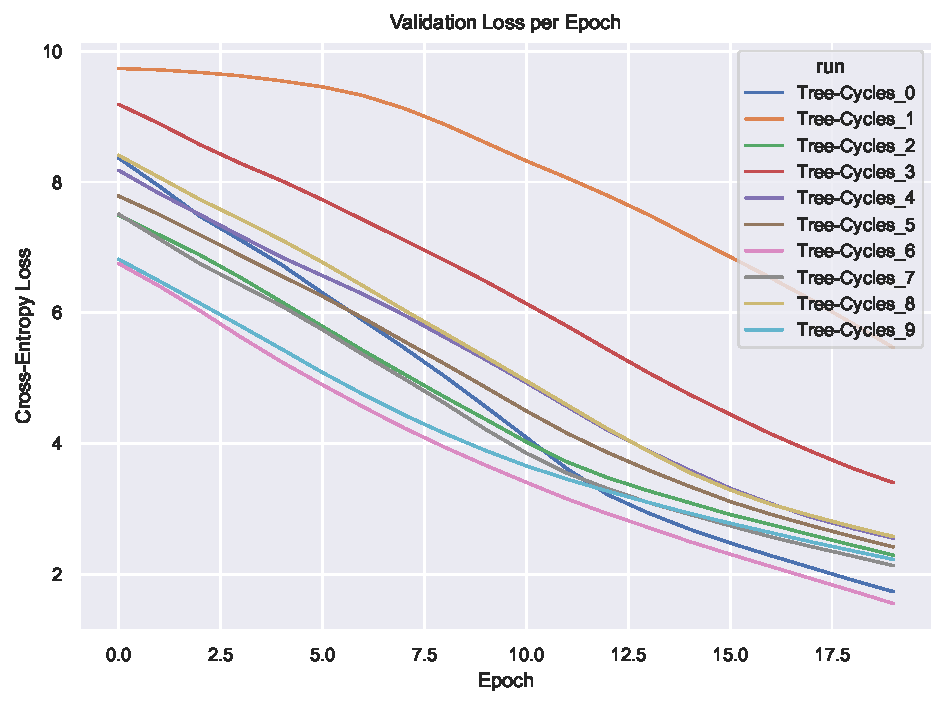
\includegraphics[width=\textwidth]{img/plots/val_loss_plot.pdf}  % Plot 1
        \caption{Mean validation Loss per Epoch (Tree-Cycles).}
        \label{fig:Tree-Cycles-val_loss}
    \end{minipage}
    \hfill
    \begin{minipage}{0.48\textwidth}
        \centering
        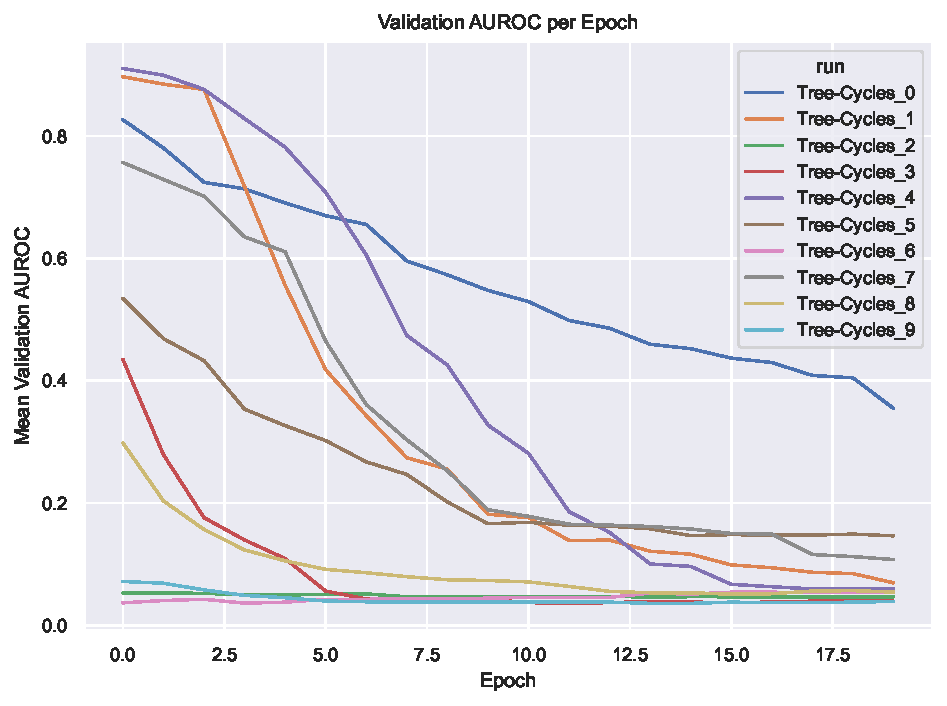
\includegraphics[width=\textwidth]{img/plots/val_auroc_plot.pdf}  % Plot 2
        \caption{Mean validation AUROC per Epoch (Tree-Cycles).}
        \label{fig:Tree-Cycles-val_auroc}
    \end{minipage}
\end{figure}

TREE-GRID DOES NOT PERFORM WELL ON METRIC IN INDUCTIVE SETTING, CLOSE TO RANDOMNESS. QUALITATIVE RESULTS HOWEVER LOOK QUITE PROMISING. RESULTS ACHIEVED IN COLLECTIVE SETTING ALSO ALMOST IDENTICAL TO THE ONES ACHIEVED IN THE REPLICATION PAPER. USAGE OF ALL MOTIF NODES LEADS TO k-HOP GRAPHS THAT DO NOT CONTAIN COMPLETE MOTIF! LEADS TO EXPLANATION ONLY CONTAINING 3 "BOXES" OF THE 4, AS SEEN IN BAD PERFORMING MODELS?
DURING OUR TRAINING: 11 of 30 training instances consisted of only motif nodes/edges, resulting in an incomputable AUROC
NOTABLE THAT LOSS DOES CONVERGE 

\begin{figure}[htbp]
    \centering
    \begin{minipage}{0.48\textwidth}
        \centering
        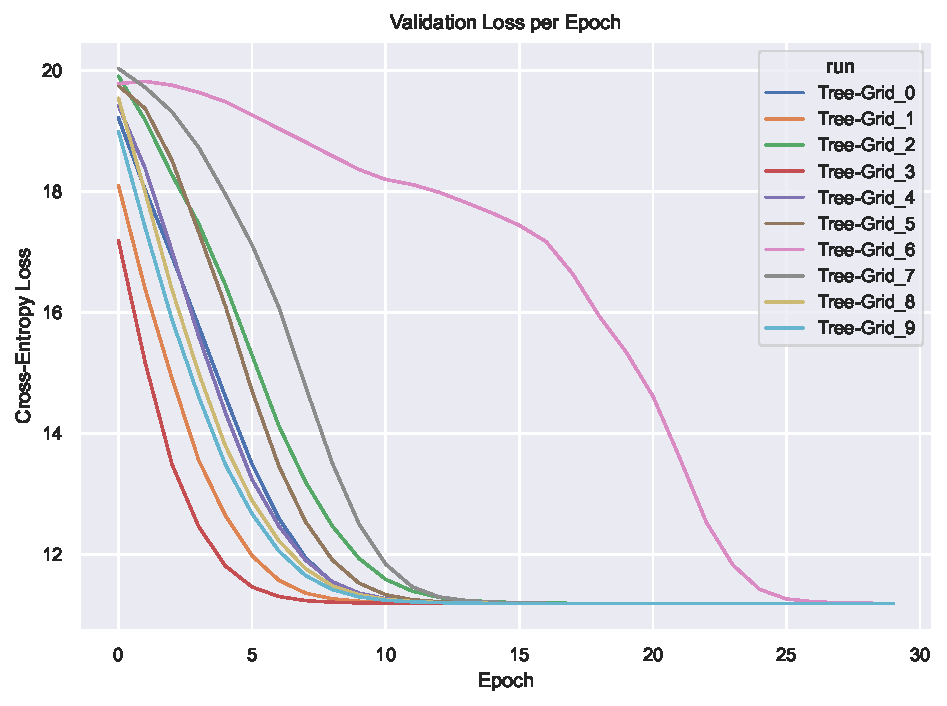
\includegraphics[width=\textwidth]{img/plots/Grid_val_loss_plot.pdf}  % Plot 1
        \caption{Mean validation Loss per Epoch (Tree-Grid).}
        \label{fig:Tree-Grid-val_loss}
    \end{minipage}
    \hfill
    \begin{minipage}{0.48\textwidth}
        \centering
        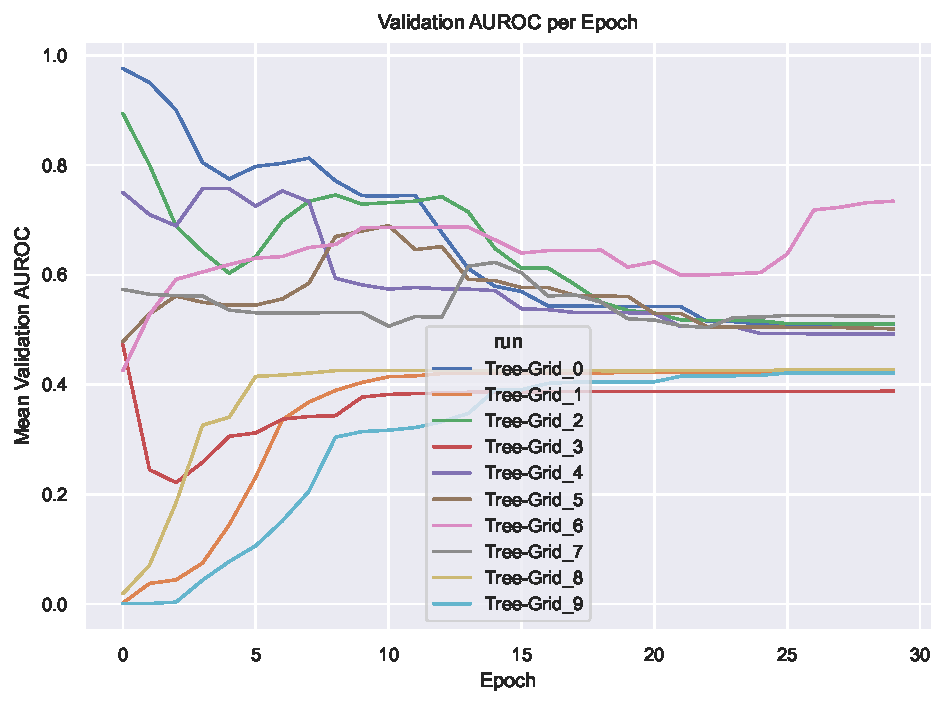
\includegraphics[width=\textwidth]{img/plots/Grid_val_auroc_plot.pdf}  % Plot 2
        \caption{Mean validation AUROC per Epoch (Tree-Grid).}
        \label{fig:Tree-Grid-val_auroc}
    \end{minipage}
\end{figure}

\begin{figure}[htbp]
    \centering
    \begin{minipage}{0.48\textwidth}
        \centering
        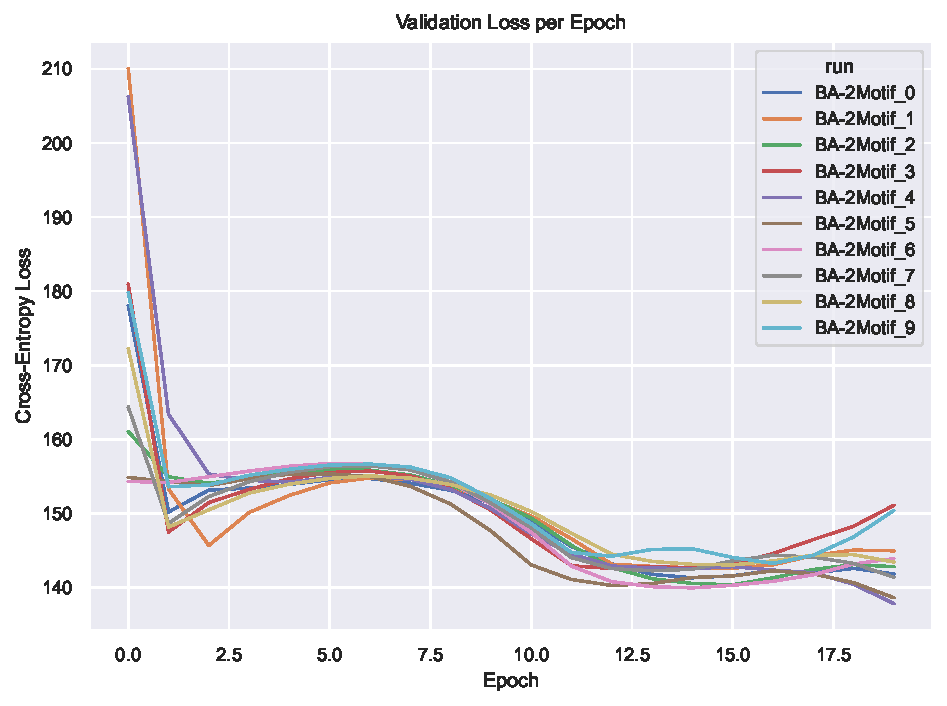
\includegraphics[width=\textwidth]{img/plots/2M_val_loss_plot.pdf}  % Plot 1
        \caption{Mean validation Loss per Epoch (BA-2Motif).}
        \label{fig:BA-2Motif-val_loss}
    \end{minipage}
    \hfill
    \begin{minipage}{0.48\textwidth}
        \centering
        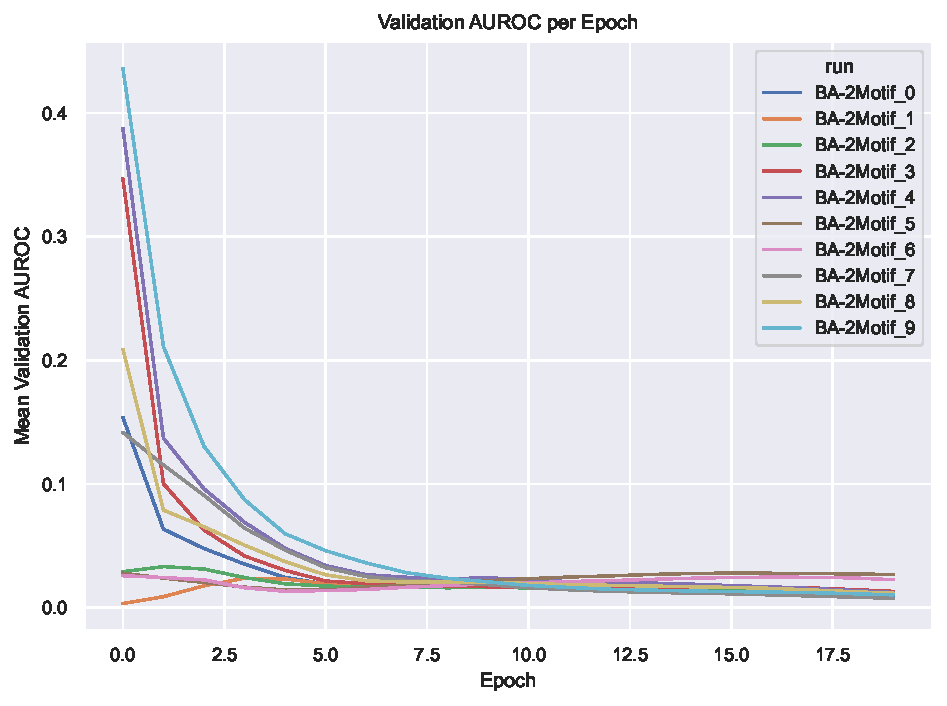
\includegraphics[width=\textwidth]{img/plots/2M_val_auroc_plot.pdf}  % Plot 2
        \caption{Mean validation AUROC per Epoch (BA-2Motif).}
        \label{fig:BA-2Motif-val_auroc}
    \end{minipage}
\end{figure}


%We use normalization in our downstream models, though it is not described in the paper, since it is used in the code. We also experimented with the effects of the use of normalization since it seems to be relevant to the performance of the explainer. \\

%It is important to highlight that our code achieved better and way more stable results for BA-2Motif when trained on a gpu instead of cpu. \\
%Ba-Shapes, Tree-Cycles and MUTAG results achieved were identical. \\
%Ba-Community and Tree-Grid achieved very slightly better results on CPU. \\

%Sweeps: (Params ordered by importance)\\
%BA-Shapes: higher size reg -> 0.1; lower entropy reg -> 0.01; lr and tT very low impact but slightly higher -> 0.01 and 5. Note that Loss curve jumps on most runs! (logical-sweep-94 and restful-sweep-92 have clean loss) TRY HIGHER SIZE REG AND LOWER ENTROPY REG \\

%BA-Community: lr 0.0001 too low, not working -> 0.003; lower entropy -> 0.1; higher size -> 0.1; TRY MORE SEEDS, LR, EPOCHS? \\

%Tree-Cycles: high lr -> 0.01 ; lower entropy reg -> 0.1/0.01; higher size reg -> 0.1/0.01 ; lower tT -> 1. TRY WITH MORE SEEDS FOR ENT, SIZE, TEMP? Confirmed higher size reg -> 0.1; lower entropy reg -> 0.01; temp really low impact, tendency higher. TRY 30 EPOCHS???\\

%Tree-Grid: high lr -> 0.01; high size reg -> 1; higher entropy reg? -> 10/1, high tT -> 5. TRY MORE SEEDS FOR ENTROPY REG -> not quite clear, tendency lower; MAYBE EVEN HIGHER LR -> No\\

%BA-2Motif: RUN ON GPU - Not the cause. Cause for better results were features of 1 instead of 0.1! However, good results achieved on BA2-Motif dataset from pyg, not original one.\\

%MUTAG: Low lr -> 0.0003; low entropy reg(high impact, but highest AUC runs vary) -> 0.1; low tT -> 1; less epochs -> 20; low size reg -> 0.005(/0.01); Loss is messy and AUC seems to decrease over time! lr 0.0001 worse, entropy reg 0.1/0.01 has zero effect -> 0.1\\

\subsection{Collective Setting}

\textbf{Experimental Setup} \par
To allow for a better comparison with both baselines we perform an experiment in the collective setting. Therefore, both the training and evaluation are performed on the complete set of motif instances. This is the setting that can be found in the original codebase. It is noteworthy that we use the hyperparameters found in an inductive setting (see Section \ref{}), which should allow for good generalization. We also include our results obtained in the inductive setting, to evaluate the difference between the settings. \bigskip

\textbf{Results}\par

We cannot reproduce the scores achieved in the original work for most of the datasets, as seen in Table \ref{}. BA-Shapes achieves a higher score than the original, while MUTAG comes close to the original baseline and even obtains a higher score in the inductive setting. The other scores do not come close when considering the scores as they are without flipped ground truths. We are however able to match the results achieved in the RE-PGExplainer baseline, in all but Tree-Cycles. This validates that the PGExplainer is applicable to different downstream GNN architectures.

\begin{table}[ht]
    \centering
    \scriptsize
    \begin{tabularx}{\textwidth}{l|XXXX|XX}   % 'X' column type from tabularx automatically scales columns
    \textbf{} & \multicolumn{4}{c}{\textbf{Node Classification}} & \multicolumn{2}{c}{\textbf{Graph Classification}} \\
    \textbf{Method} & BA-Shapes & BA-Community & Tree-Cycles & Tree-Grid & BA-2Motif & MUTAG \\
    \midrule
    \addlinespace
    \textbf{} & \multicolumn{6}{c}{\textbf{Explanation AUC}} \\
    \midrule
    PGExplainer & 0.963$\pm$0.011 & 0.945$\pm$0.019 & 0.987$\pm$0.007 & 0.907$\pm$0.014 & 0.926$\pm$0.021 & 0.873$\pm$0.013 \\
    \midrule
    RE-PGExplainer & 0.999$\pm$0.000 & 0.825$\pm$0.040 & 0.760$\pm$0.014 & 0.679$\pm$0.008 & 0.133$\pm$0.046 & 0.843$\pm$0.084 \\
    \midrule
    Our work & 0.993$\pm$0.001 & 0.831$\pm$0.009 & 0.084$\pm$0.078 & 0.679$\pm$0.032 & 0.018$\pm$0.004 & 0.833$\pm$0.006 \\
    \midrule
    %collective with Xavier & 0.993.$\pm$0.003 & 0.833$\pm$0.023 & 0.322$\pm$0.278 & 0.68$\pm$0.057 & 0.027$\pm$0.009 & 0.774$\pm$0.034 \\
    %\midrule
    \midrule
    Our work (inductive) & 0.994$\pm$0.001 & 0.754$\pm$0.013 & 0.106$\pm$0.104 & 0.537$\pm$0.081 & 0.017$\pm$0.006 & 0.874$\pm$0.009 \\
    \bottomrule
    \end{tabularx}
    \caption[Collective performance of our reimplementation]{Collective PGExplainer performance in Explanation AUROC ($a=N$).}
    \label{tab:pgexplainer_auc}
\end{table}


\subsection{Inductive Setting with more training data}

\textbf{Experimental Setup}\par
Luo et al. \cite{} show that the inductive performance of PGExplainer improves with the number of instances used for training. To validate this we perform an inductive experiment with an increase number of training instances $a=60$. Since the motif instance sets of BA-Shapes and Tree-Cycles in the original setting only consist of 60 instances, we use a percental split of $0.8/0.1/0.1$. This leads to $a=48$ for these two tasks. \bigskip

\textbf{Results}\par
Table \ref{tab:experiment_60train}

BA-Community: SumSampledEdges increases after 6/7 epochs, AUROC reaches peak early but then decreases steadily! (For 30 instances: Both sum sampled edges and AUROC converge very strongly!) - Apparently less stable on 60 instances (ONLY CHANGE!!!), probably would have to be retuned (BAD!)
\begin{table}[ht]
    \centering
    \scriptsize
    \begin{tabularx}{\textwidth}{l*{6}{X}}   % 'X' column type from tabularx automatically scales columns
    \toprule
    \textbf{} & \multicolumn{6}{c}{\textbf{Explanation AUC}} \\
    \cmidrule{2-7}
    \textbf{Method} & BA-Shapes & BA-Community & Tree-Cycles & Tree-Grid & BA-2Motif & MUTAG \\
    \midrule
    Our work (inductive) & 0.994$\pm$0.001 & 0.754$\pm$0.013 & 0.106$\pm$0.104 & 0.537$\pm$0.081 & 0.017$\pm$0.006 & 0.874$\pm$0.009 \\
    \midrule
    with Xavier & 0.995$\pm$0.002 & 0.779$\pm$0.036 & 0.467$\pm$0.316 & 0.551$\pm$0.119 & 0.035$\pm$0.05 & 0.834$\pm$0.04 \\
    \midrule
    $a=60$ & 0.987$\pm$0.002 & 0.641$\pm$0.045 & 0.144$\pm$0.096 & 0.495$\pm$0.052 & 0.017$\pm$0.004 & 0.895$\pm$0.009 \\
    \bottomrule
    \end{tabularx}
    \caption[Inductive performance with 60 training instances]{PGExplainer performance in Explanation AUROC ($a=60$) (He initialized).}
    \label{tab:experiment_60train}
\end{table}

\subsection{BA-2Motif with flipped GT}

\textbf{Experimental setup}
Since we found that the AUROC metric for BA-2Motif decreases rather than increases over the training epochs, and converges near zero, we run an additional experiment with flipped GT. Since both the loss and AUROC curves decrease steadily and flatten in the original inductive experiment, we consider this experiment an additional validation.
The mean individual AUROC is calculated identical to before, but the ground truth mask of each graph is inverted, meaning that edges in the motif now carry a label of $0$ and all other edges a label of $1$. 
Note that the ground truth does not affect the training procedure in any way and merely changes the metric evaluation. \bigskip

\textbf{Results}

As expected, the AUROC score for BA-2Motif is nearly perfect in this experiment, even higher than in the original work, as seen in Table \ref{tab:flippedGT}. It is notable that the results by Holdijk et al. suggest a similar observation, however the authors do not expand on this.

\begin{table}[ht]
    \centering
    \scriptsize
    \begin{tabularx}{0.4\textwidth}{l c}
        \toprule
        \textbf{Method} & \textbf{Explanation AUC} \\
        \midrule
        PGExplainer       & 0.926$\pm$0.021 \\
        RE-PGExplainer       & 0.133$\pm$0.046 \\
        Our work       & 0.017$\pm$0.006 \\
        \midrule
        Flipped GT     & 0.985$\pm$0.006 \\
        \bottomrule
    \end{tabularx}
    \caption[Inductive performance on BA-2Motif with flipped ground truth]{Explanation AUROC for BA-2Motif with flipped GT.}
    \label{tab:flippedGT}
\end{table}

\subsection{Effects of used Motif Instances}
\label{sec:motif_set_experiment}

We conduct an experiment on the performance with only select motif nodes! only taking 30 random nodes from all motif nodes may lead to a selection of mostly nodes where not even the complete motif, and even less probable edges outside the motif, are contained.

Therefore, we change the motif nodes that are used for training/evaluating to include all or one select motif node, depending on the dataset. We use the same hyperparameters used for the previous experiments. Besides this change, we follow the experimental setup to evaluate whether a reasoning behind the node selection can be made out.

\textbf{Experimental setup}

He initialized

AllMotifNodes experiment:
BA-Shapes: All house nodes (300 nodes)
Tree-Cycles: All Cycle nodes (360 nodes)
\bigskip


OneMotifNode experiment:

BA-Community:
\begin{verbatim}
    middleCommNodes = [i for i in range(single_label.shape[0]) 
            if single_label[i] == 1 or single_label[i] == 5]
    singularNodes = [_ for i,_ in enumerate(middleCommNodes) if i%2 == 0]
\end{verbatim}
(One of the two middle house nodes) (160 nodes)

Tree-Grid:
[512,800,9]
(One of the two nodes that connect to the base connection node for each motif, to contain full motif) (32 nodes)

Maybe works well because if all motif nodes are used, subgraphs are used where only the motif or even only part of the motif is present (Tree-Grid). Thus constantly using one singular same node that contains the complete motif may be better?


\textbf{Results}

OneMotifNode trivializes the problem?!

AllMotifNodes seems reasonable, since we want to be able to explain as many nodes as possible!

Further idea: Use a subset of the static one motif nodes for training and evaluate using all motif nodes?

\begin{table}[ht]
    \centering
    \scriptsize
    \begin{tabularx}{0.6\textwidth}{l*{2}{X}}   % Adjust width as needed
    \toprule
    \textbf{} & \multicolumn{2}{c}{\textbf{Explanation AUC}} \\
    \cmidrule{2-3}
    \textbf{Method} & BA-Shapes & Tree-Cycles \\
    \midrule
    Our work & 0.994$\pm$0.001 & 0.106$\pm$0.104 \\
    \midrule
    AllMotifNodes & 0.959$\pm$0.004 & 0.204$\pm$0.162 \\
    \midrule
    AllMotifNodes Xavier & 0.948$\pm$0.015 & 0.247$\pm$0.197 \\
    \bottomrule
    \end{tabularx}
    \caption[Inductive performance using all motif nodes for training]{Explanation AUROC for AllMotifNodes on selected datasets.}
    \label{tab:allmotifnodes_selected}
\end{table}

\begin{table}[ht]
    \centering
    \scriptsize
    \begin{tabularx}{0.6\textwidth}{l*{2}{X}}   % Adjust width as needed
    \toprule
    \textbf{} & \multicolumn{2}{c}{\textbf{Explanation AUC}} \\
    \cmidrule{2-3}
    \textbf{Method} & BA-Community & Tree-Grid \\
    \midrule
    Our work & 0.754$\pm$0.013 & 0.537$\pm$0.081 \\
    \midrule
    OneMotifNode & 0.951$\pm$0.007 & 1.0$\pm$0.0 \\
    \bottomrule
    \end{tabularx}
    \caption[Inductive performance using one motif node for training]{Explanation AUROC for OneMotifNode on selected datasets.}
    \label{tab:allmotifnodes_selected}
\end{table}


\begin{table}[ht]
    \centering
    \scriptsize
    \begin{tabularx}{0.6\textwidth}{l*{4}{X}}   % Adjust width as needed
    \toprule
    \textbf{} & \multicolumn{4}{c}{\textbf{Explanation AUC}} \\
    \cmidrule{2-5}
    \textbf{Method} & BA-Shapes & BA-Community & Tree-Cycles & Tree-Grid \\
    \midrule
    Experiment & 0.85$\pm$0.005 & 0.731$\pm$0.016 & 0.224$\pm$0.160 & 0.65$\pm$0.026 \\
    \bottomrule
    \end{tabularx}
    \caption[Inductive performance using one motif node for training and all other motif nodes for evaluation]{Explanation AUROC when training with a subset of one node per motif and evaluating on all motif nodes for node tasks.}
    \label{tab:allmotifnodes_selected}
\end{table}

\subsection{Qualitative Analysis}

\textbf{Experimental setup}

Top 5 edges were taken for BA-2Motif, as done in original. This accounts for all edges of the circle motif and 5 of the 6 edges in a house motif.

For MUTAG the top 10 edges are selected, as the authors state that the shared base motif is also learned.

For Tree-Cycles and BA-2Motif the lowest AUROC models were used and the top-k lowest edges were sampled.

\textbf{Results}

We found that the MUTAG explainer detects the chemical combinations that cause the mutagenicity as the highest edge quite often, but the shared base ring is not detected at all. The explainer detects the general 2 element combinations over the rings?


%\subsection{Training on ALL instances - Evaluation only on motif instances?}
%This probably would not grant any insights, since training on non motif nodes should in theory mostly lead to all edges being irrelevant for prediction?? Bascially most edge could be removed and in theory the prediction of the node should not change at all, therefore no information can be gather from this?

%\textbf{Experimental setup}

%\textbf{Results}

\subsection{BA-2Motif with wrong features}
- Effects of using "wrong" node features for downstream task?

Comparison to orginal one: Original dataset transformed to pytorch performs way worse, for features of 0.1! Mean AUC of about 0.4! \\
Original dataset with features changed to ones instead of 0.1: Works good as well.



\section{PGExplainer applied to NeuroSAT}
\label{sec:SAT-experiments}

TODO: We present our approach for generating bipartite explanations for NeuroSAT \cite{} predictions of SAT problems.

\subsection{Common experimental setup}

NeuroSAT \cite{selsam2018learning} uses a distribution $\textbf{SR}(n)$ that creates pairs of SAT problems on $n$ variables, which are satisfiable and unsatisfiable, only differing in a singular negated literal. These are created by randomly sampling subclauses of $k$ variables, where each variable is negated with a probability of $50\%$. These subclauses are added to the problem until a SAT solver \cite{een2003extensible} finds it to be unsatisfiable. We adapt this to only contain singular unsatisfiable problems, rather than pairs of problems, since UNSAT cores only appear in unsatisfiable problems. The difficulty of the problems is slightly reduced by using $n=8$, to allow for the explainer to run on NeuroSAT on our limited hardware. We create a dataset of 100 problems.

We create the expected ground truth with the deletion-based MUS extractor \verb|MUSX| from PySAT \cite{imms-sat18}, as described in section \ref{sec:Application_to_NeuroSAT}.

The quantitative evaluation is adopted from Section \ref{sec:PGE_exp_setup}, with the positive targets being the edges that appear in the corresponding ground truth MUS of each problem. Since the qualitative evaluation relies on knowing $k$, we calculate this dynamically during evaluation from the ground truth of the current problem.

The NeuroSAT model was provided by a fellow student, trained on a $\textbf{SR}(40)$ distribution. It achieves an accuracy of 1.0 on the dataset we created.

We apply PGExplainer in the inductive setting, using a 50/25/25 split for training, evaluating and testing the NeuroSAT explainer. \bigskip

\textbf{Hyperparameter Search}\par
We perform a hyperparameter search for both the explainer with the soft constraint, and the explainer with the applied hard constraint. We follow the general grid search procedure used for the previous experiments, but introduce three new hyperparameters, one exclusive to the hard constraint and one exclusive to the soft constraint. $\alpha_{arch} \in \{0,1\}$, exclusive to the hard constraint, denotes whether a more complex MLP architecture is used in the explainer. The second introduced hyperparameter $\alpha_{concat} \in \{0,1\}$ controls whether the node embeddings $\mathbf{z}$ are used from the last iteration of NeuroSAT or if a concatenation of the states at multiple iterations shall be used (see Section \ref{sec:NeuroSAT_extension}). TODO: HYPERPARAM ADAMW TO CONTROL WETHER ADAMW(0.01) OR ADAM WITHOUT WEIGHT DECAY IS USED. Lastly, the coefficient $\alpha_{c} \in \mathbb{R}^+$ controls the effect of the soft constraint $R_C$ (see Equation \ref{eq:soft_restraint}) on the loss. This is disregarded in the hard constraint experiment, as the hard constraint replaces the soft constraint. The sample bias $b$ used in PGExplainer is disregarded completely. We found that the validation AUROC tends to decrease during training and therefore focus on minimizing the metric as well as the validation loss. TODO: Also consider highest individual local AUROC


\subsection{Soft Constraint Experiment}
In this experiment we adopt the soft constraint introduced in Section \ref{sec:NeuroSAT_extension} to use the PGExplainer to generate explanations for the predictions of NeuroSAT on unsatisfiable SAT problems. \bigskip

\textbf{Results}\par


\subsection{Hard Constraint Experiment}
In this experiment we adopt the hard constraint introduced in Section \ref{sec:NeuroSAT_extension} to use the PGExplainer to generate explanations for the predictions of NeuroSAT on unsatisfiable SAT problems. \bigskip

\textbf{Hyperparameter search}\par
We perform a hyperparameter search for both the explainer with the soft constraint, and the explainer with the hard constraints. We follow the general grid search procedure used for the previous experiments, but introduce new hyperparameters. 

The search revealed that none of the parameter configurations achieves an AUROC score above $0.5$ and below $0.44$. Since $0.5$ equals pure randomness and is usually caused by all edges being predicted with a score of $0$, we select the model that achieves the lowest score, thus departing from the point of randomness. However, this mostly indicates that the explainer predictions do not align with the selected ground truth. We found that a low learning rate is important to keep the edge predictions from reaching 0, as these steadily decrease over training time. $\alpha_s=1.0$ further enhanced this unwanted behavior. Using a concatenation of the embedding at multiple iterations achieved worse results than the usual graph task procedure when considering the highest individual AUROC of a validation instance. However, this does not consider whether a general procedure is learned.

\textbf{Results}\par
We found that running the training for 500 epochs resulted in a converging loss, as well as a converging metric score, close to $0.46$. A local score minimum is reached in epoch 60 with a value of $0.44$. Since this is very close to a score indicating randomness, we conclude that NeuroSAT does in fact not learn generalized unsatisfiable cores in the form of MUSs.